\documentclass[conference]{IEEEtran}

\usepackage{silence}
\WarningsOff[latexfont]

\usepackage{amsmath}
\usepackage[american]{babel}
\usepackage{booktabs}
\usepackage{multirow}
\usepackage[noabbrev,capitalise]{cleveref}
\usepackage[T1]{fontenc}
\usepackage[utf8]{inputenc}
\usepackage[binary-units,per-mode=symbol]{siunitx}
\usepackage[caption=false,font=footnotesize]{subfig}
\usepackage{xfrac}
\usepackage{xspace}

\begin{document}

\title{Parameters evaluation of abstract web objects}

\author{
    \IEEEauthorblockN{Alessandro Pezzé, 182501}
    \texttt{alessandro.pezze@studenti.unitn.it}
}

\maketitle

\begin{abstract}
Starting from 10 sets of web objects, possibly representing advertisements linked to browsing generic web pages, and their associated metrics, which are their number of downloads and their revenue generated in a way we are not concerned with, analyse each set in order to find out the values of hidden parameters which rules how the system works, estimate the confidence interval about one of these parameters and plot significant data.
\end{abstract}

\section{Introduction}\label{sec:introduction}

A system of revenue per download is defined by a known function with some hidden parameters.  Those parameters are inferred by analysing the data and applying to it common formulas and calculations.

\section{Fundamentals}\label{sec:fundamentals}

We are presented with ten sets of web objects, each set comprises 2400 objects which are defined by two metrics which are: \(x_i(t)\) the number of downloads of the i-th object at time t, \(y_i(t)\) the real revenue gained by the i-th object at time t. \(x_i(t)\) is a non-decreasing cumulative function affected by noise following \(U(0,D_i^{max})\), which is a Uniform distribution between 0 and \( D_i^{max}\) which has to be inferred. 
Moreover, it is safe to say that we can derive the function of the estimated revenues from the two metrics mentioned above so that a revenue can be considered as \(y_i(x_i)\). Such function is known a priori to be linear and we also know that there is some kind of noise which affects the real values of the revenue in a form of Gaussian distribution, that Gaussian noise is moreover known to be independent to the observed object. The estimated revenue so can be seen as the \cref{eq:system}
\begin{equation}
    r_i(t) = \alpha_id_i(t-1) + \alpha_iU(0,D_i^{max}) + N(0,\sigma^2)\label{eq:system}
\end{equation}
Which says that the calculated revenue is governed by three unknown parameters which are \(\alpha_i\), \(D_i^{max}\) and \(\sigma^2\).
\(D_i^{max}\) will be estimated statistically by calculating the probability that a never happened event could occur after n iterations in a space of \(k\) variables (all the possible download increments from \(0\) to \(D_i^{max}\)) using the probability formula as shown in \cref{eq:probability}
\begin{equation}
    p = \left({k-1 \over k}\right)^n\label{eq:probability}
\end{equation}
\(\alpha_i\) can be considered from \cref{eq:system} as the slope of the line derived from that equation and thus will be estimated by fitting the revenues over the downloads while minimizing the mean square error between real data points.
\(\sigma^2\) is the variance of the Gaussian distribution found in equation \cref{eq:system} that can be approximated to a t-student distribution when the dataset is smaller than 30 individuals. The sample variance of a t-student distribution is equation \cref{eq:sigmaestimator} which will thus be used to calculate this value.
\begin{equation}
    s^2 = \sqrt{{1 \over n-1}\sum_{i=1}^n(x_i-\overline{x})^2}\label{eq:sigmaestimator}
\end{equation}
Moreover, the confidence interval of \(\sigma^2\) must be calculated using the known mean’s confidence interval for t-student distribution with a population on \(n\) values and \(n-1\) degrees of freedom as depicted in \cref{eq:studentinterval}
\begin{equation}
    \left[\bar{X} - z_{\alpha \over 2}\sqrt{s^2 \over n-1},\quad \bar{X} + z_{\alpha \over 2}\sqrt{s^2 \over n-1}\right]\label{eq:studentinterval}
\end{equation}

\section{Implementation}\label{sec:implementation}

R was used to do all the necessary calculations to derive the unknown parameters since it provides a large group of primitives to aggregate data and permits to apply known built-in functions on it. Two steps of calculations were designed because of the conformation of the unknown parameters. The first two mentioned parameters are inherent to the sets analysed so in the end of the computation it will result in ten of both those parameters, one for each given set, the computation of these values is done firstly. The last parameter, \(\sigma^2\), is known to be the same all over the ten sets so it will be calculated taking in consideration all the data in a second step of calculations. In order to start the first step of computations the data is opportunely divided into the ten sets.
\(D_i^{max}\), the number of maximum downloads per unit time, is derived by subtracting each pair of time-contiguous number of downloads, \(\Delta d\), and taking the maximum value among the differences. To confirm the correctness of the result, \cref{eq:probability} was used to calculate the probability that \(D_i^{max} +1\) could be the largest number of maximum downloads per unit time instead of the calculated \(D_i^{max}\).
\(\alpha_i\) is the slope of the line that is formed by revenues over the number of downloads. Since these two metrics are not time continuous but a set of single pairs, linear fitting was used to derive the slope and the intercept of the hypothetical line that minimizes the error with the actual points by using the least square error function. The resulted line’s slope is then \(\alpha_i\). To reinforce the calculated result, the Pearson correlation between the two metrics, revenues and number of downloads, is calculated, showing that the two are closely tightened and follow a line path.
The estimation of \(\sigma^2\), which is the second parameter of the Gaussian distribution which affects the real revenues, is calculated by looking at the real revenues data coming from the 10 datasets, each splitted in two in order to have more samples, and the theoretical revenue values which can be found on the fitted line derived while estimating \(\alpha_i\). In order to have more samples and thus effectively use a t-student distribution instead of a Gaussian distribution, the 10 initial sets were divided in 20 disjoint sets. For each value of the revenues in the dataset was calculated the difference with the theoretical corresponding one and then with the twenty sets derived (10 sets divided in two) were formed their standard deviation was calculated. In order to calculate the confidence interval for \(\sigma^2\), its mean and its variance were calculated and fed, together with the appropriate \(z_{\alpha \over 2}\), into \cref{eq:studentinterval} giving us the confidence intervals for the desired confidence level required (0.9, 0.95, 0.98, 0.99, 0.998, 0.999).

\section{Evaluation}\label{sec:evaluation}

\begin{figure}[t]
    \centering
    \subfloat[all objects]{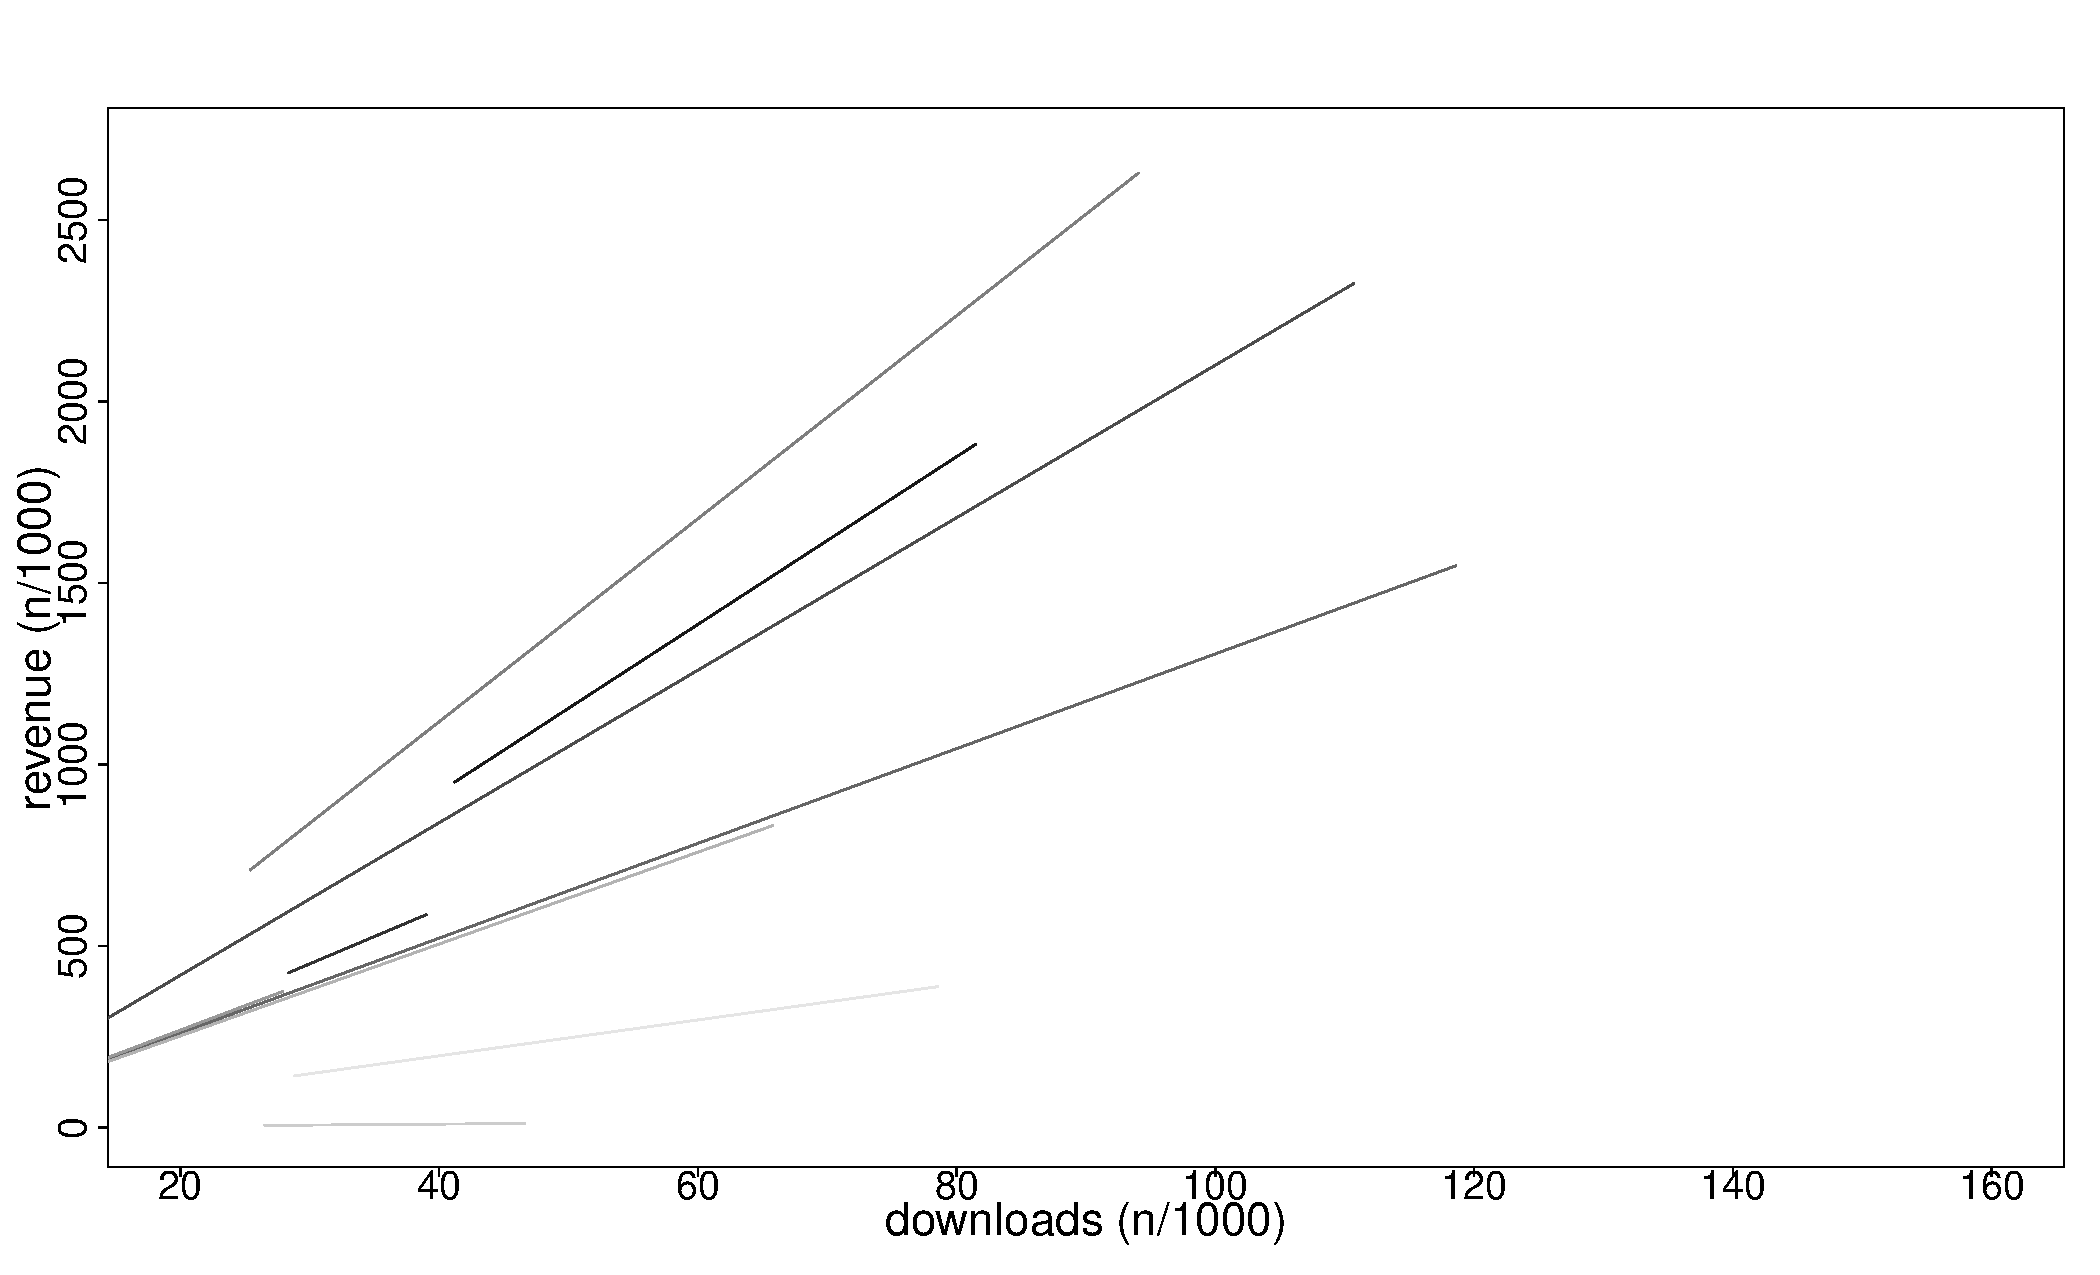
\includegraphics[width=\columnwidth]{graphs/FittedLinesTogheter}}\\
    \subfloat[object \num{7}]{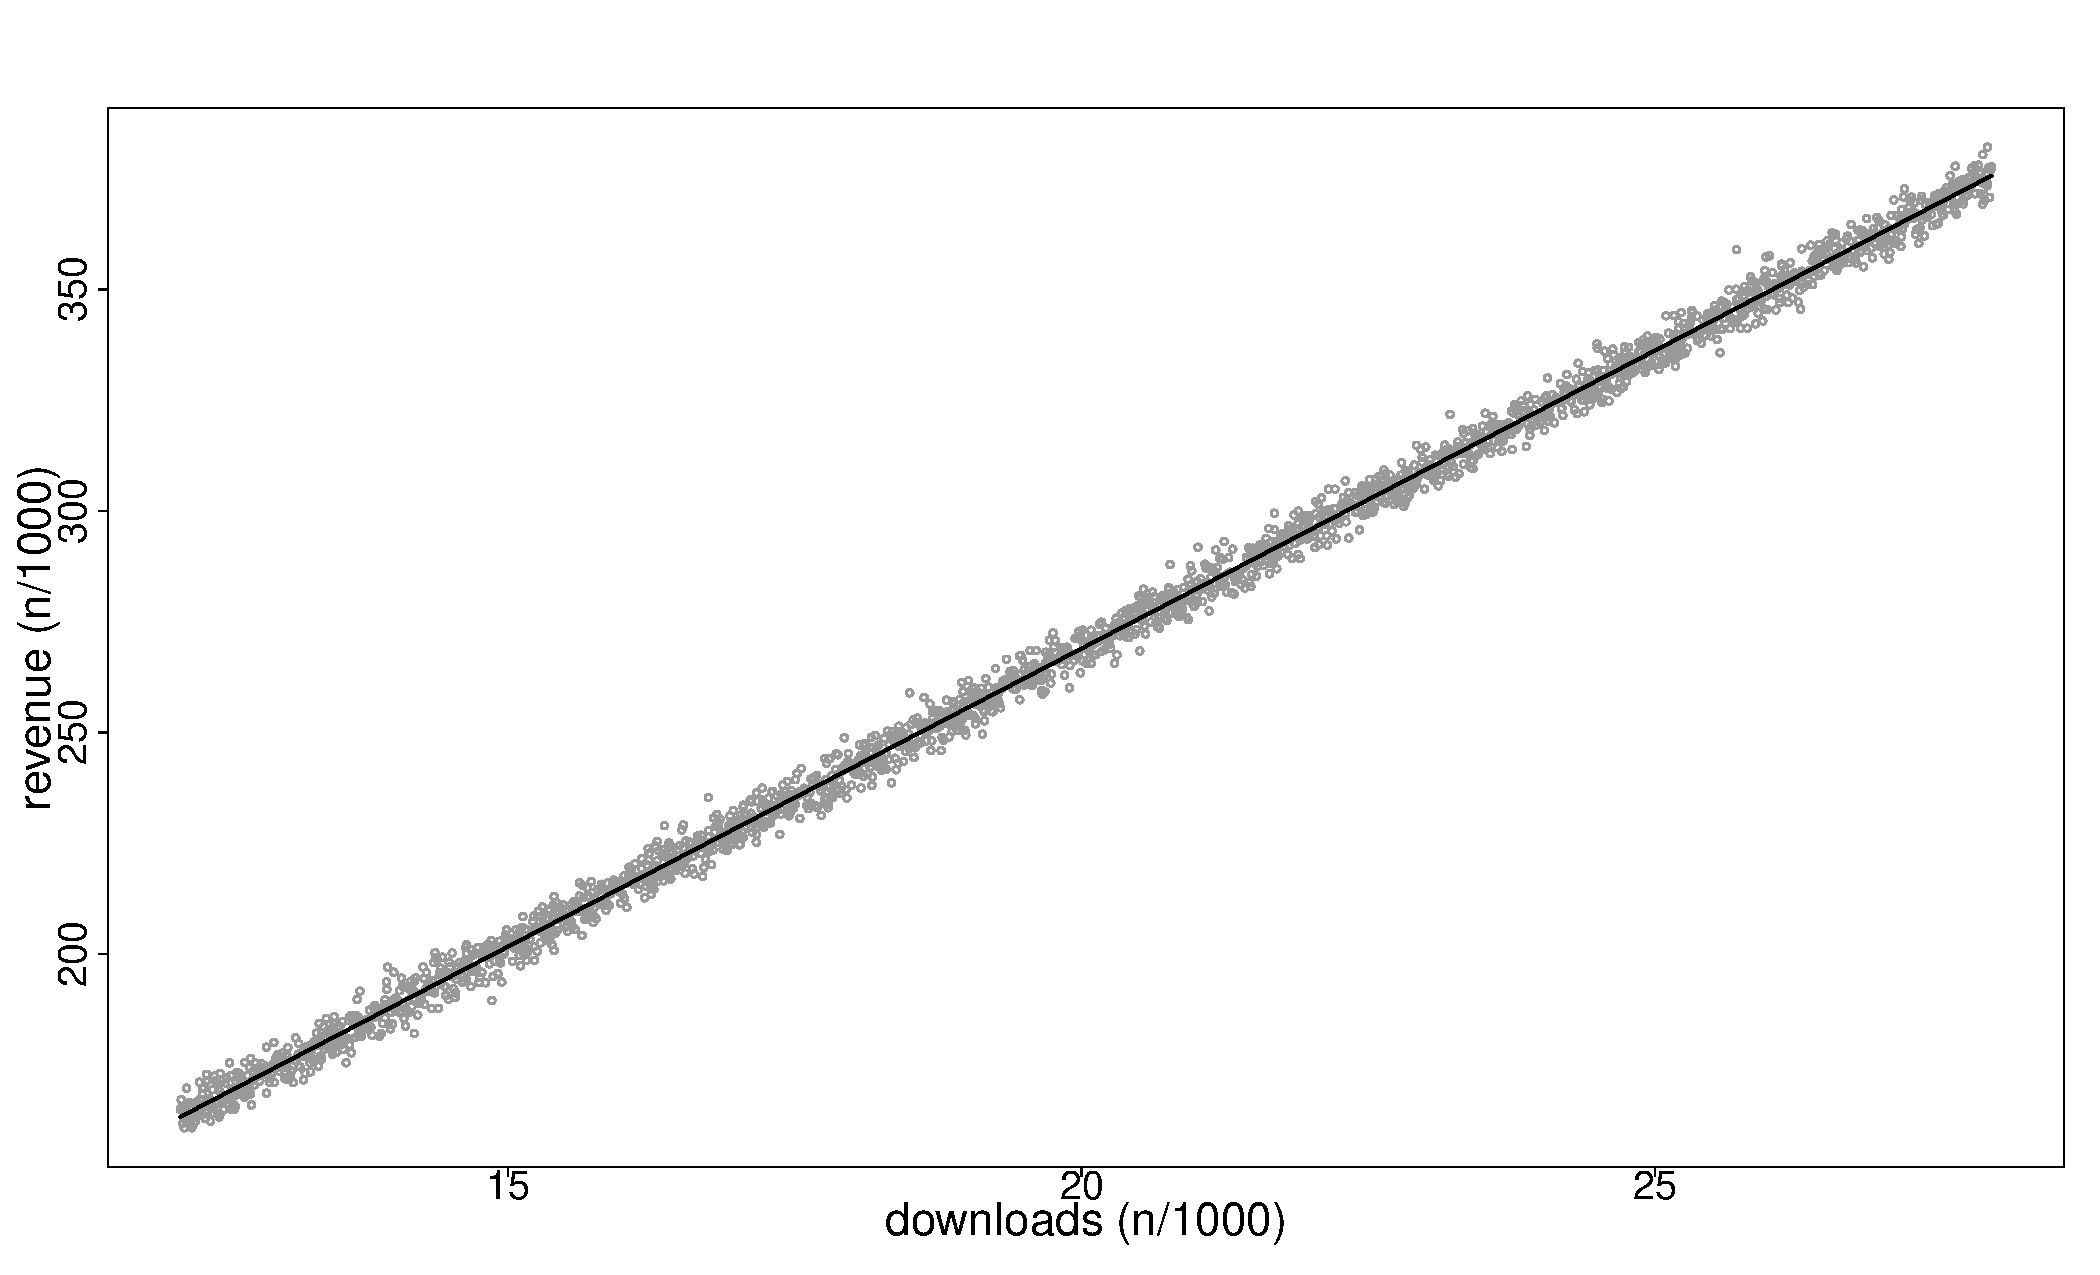
\includegraphics[width=\columnwidth]{graphs/FittedLineObject6}}
    \caption{The ten sets derived lines, a single set with scatter real data points and the linear fit}
    \label{grph:fits}
\end{figure}

\begin{figure}[t]
    \centering
    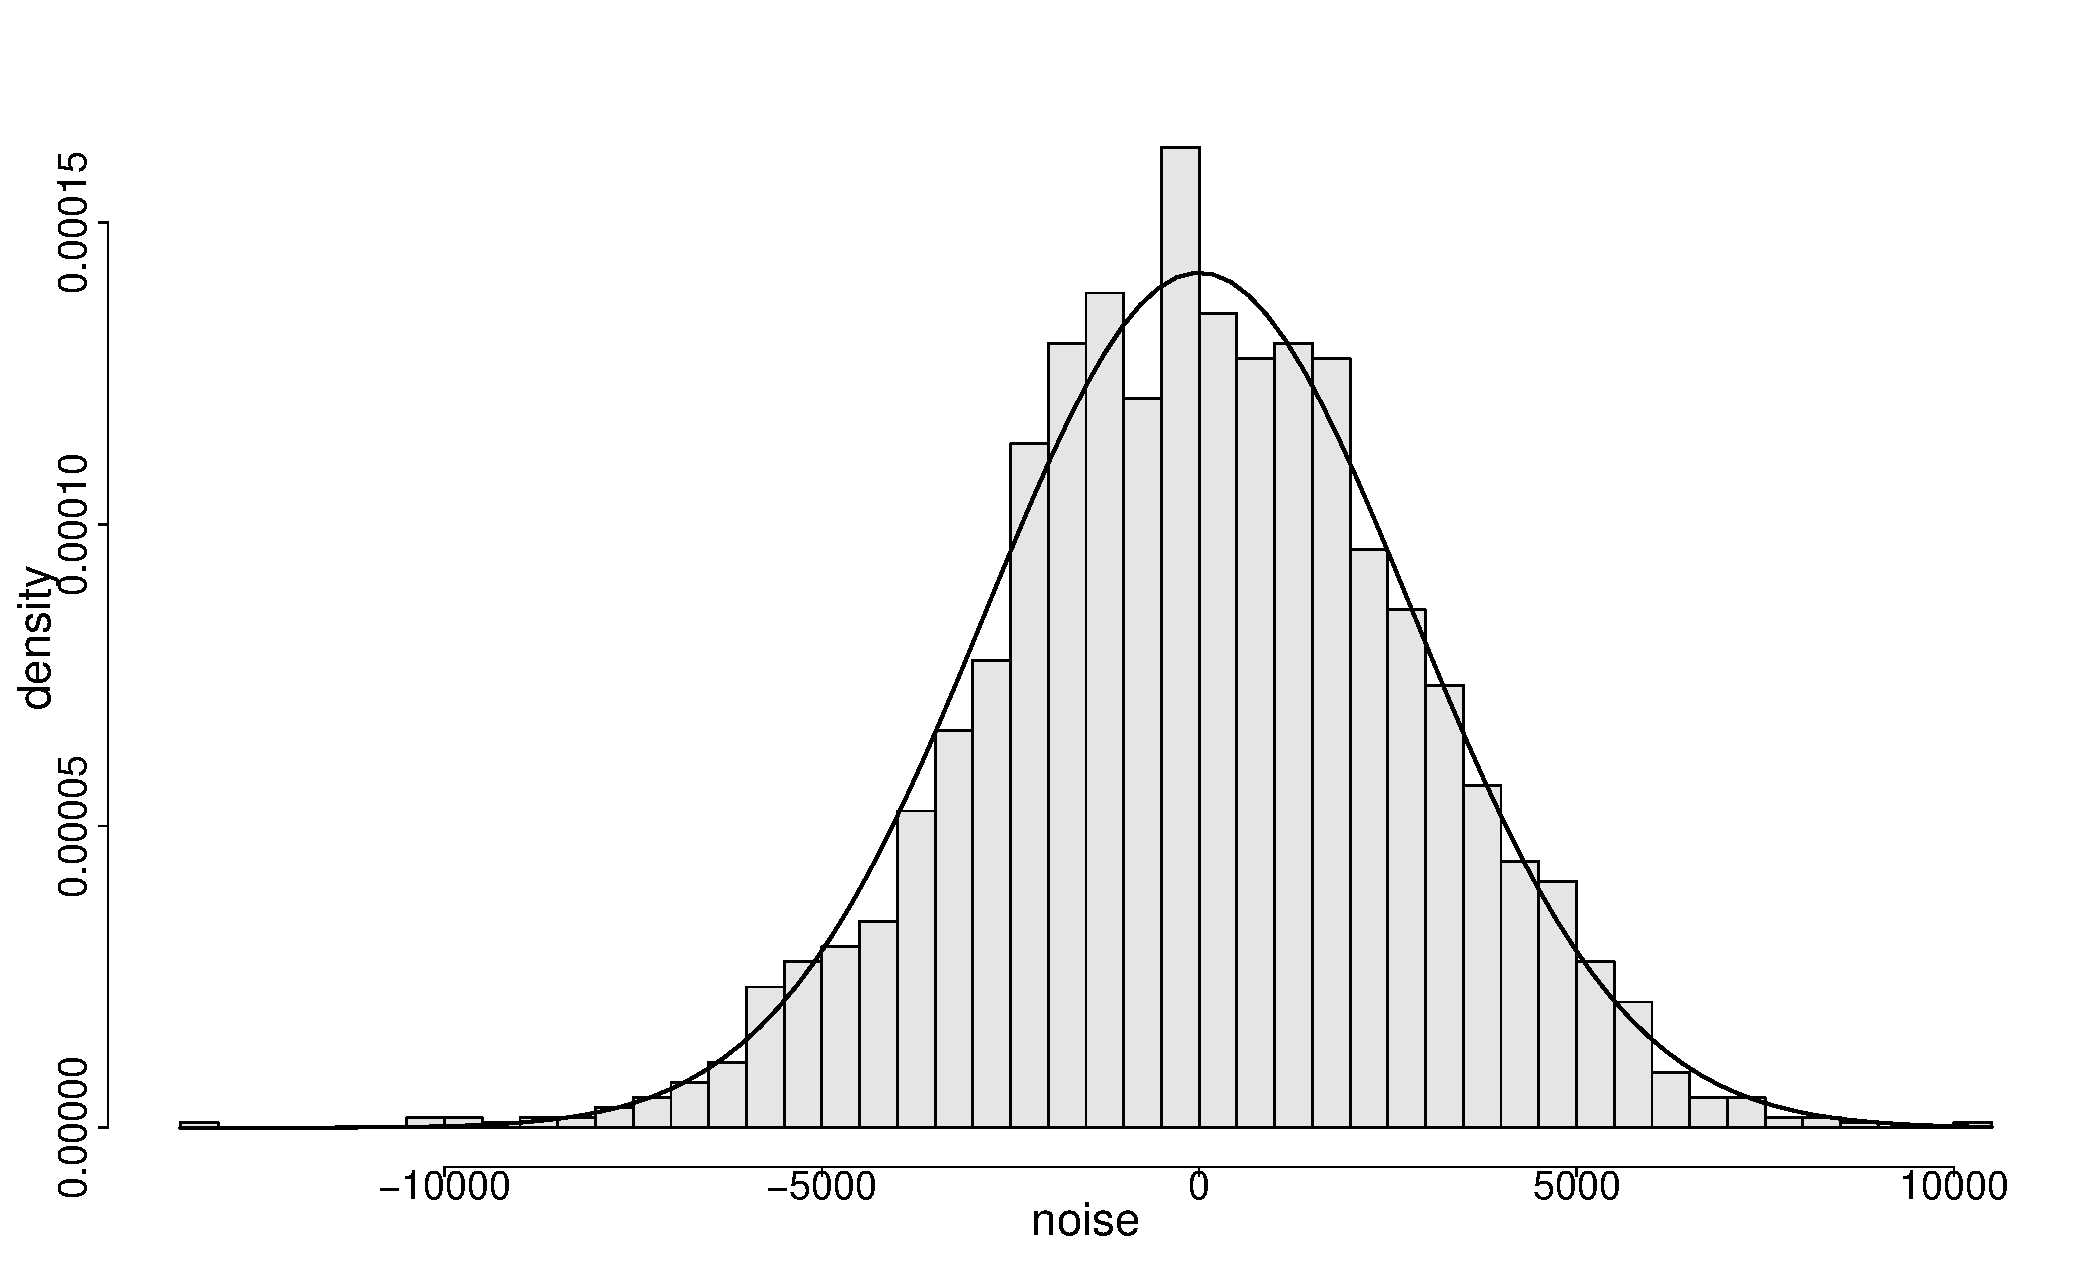
\includegraphics[width=\columnwidth]{graphs/GaussianDistribution}
    \caption{Gaussian distribution obtained from object \num{6}. The bars describe the real data grouped in bins large \(280\) elements, the curved line describe the theoretical line derived from calculations}
    \label{grph:gaussian}
\end{figure}

\begin{table}
    \centering
    \caption{\(D_i^{max}\) and \(\alpha_i\) results}
    \label{tab:resultsobjects}
    \begin{tabular}{c|cc|cc}
        \toprule
        object & \(D_i^{max}\) & error probability & \(\alpha_i\) & correlation \\
        \midrule
        \num{1} & \num{82} & \(6.290477\cdot10^{-31}\) & \num{23.094} & \num{0.999946} \\
        \num{2} & \num{80} & \(4.99975\cdot10^{-100}\) & \num{15.043} & \num{0.998311} \\
        \num{3} & \num{79} & \(4.6774\cdot10^{-13}\) & \num{20.999} & \num{0.999990} \\
        \num{4} & \num{59} & \(5.450097\cdot10^{-12}\) & \num{13.046} & \num{0.999977} \\
        \num{5} & \num{13} & \(3.084084\cdot10^{-18}\) & \num{27.947} & \num{0.999988} \\
        \num{6} & \num{86} & \(1.312886\cdot10^{-72}\) & \num{13.451} & \num{0.998952} \\
        \num{7} & \num{99} & \(1.261195\cdot10^{-23}\) & \num{12.646} & \num{0.999899} \\
        \num{8} & \num{24} & \(4.664994\cdot10^{-57}\) & \num{0.26737} & \num{0.492021} \\
        \num{9} & \num{84} & \(1.116488\cdot10^{-24}\) & \num{4.9389} & \num{0.999267} \\
        \num{10} & \num{97} & \(1.927963\cdot10^{-123}\)  & \num{7.8592} & \num{0.990403} \\
        \bottomrule
    \end{tabular}
\end{table}

\begin{table}
    \centering
    \caption{\(\sigma^2\) results (\(n = 20\))}
    \label{tab:resultssigmasplit}
    \begin{tabular}{ccc}
        \toprule
        \(\sigma^2\) & \(\sigma^2\) interval & confidence \\
        \midrule
        \multirow{6}{*}{\num{2755.3}}
         & {[}\num{2752.6}, \num{2758.0}{]} & \num{0.900} \\
         & {[}\num{2752.1}, \num{2758.5}{]} & \num{0.950} \\
         & {[}\num{2751.5}, \num{2759.1}{]} & \num{0.980} \\
         & {[}\num{2751.1}, \num{2759.6}{]} & \num{0.990} \\
         & {[}\num{2750.2}, \num{2760.4}{]} & \num{0.998} \\
         & {[}\num{2749.9}, \num{2760.7}{]} & \num{0.999} \\
        \bottomrule
    \end{tabular}
\end{table}

\begin{table}
    \centering
    \caption{\(\sigma^2\) results (\(n = 10\))}
    \label{tab:resultssigmanotsplit}
    \begin{tabular}{ccc}
        \toprule
        \(\sigma^2\) & \(\sigma^2\) interval & confidence \\
        \midrule
        \multirow{6}{*}{\num{2755.1}}
         & {[}\num{2751.9}, \num{2758.3}{]} & \num{0.900} \\
         & {[}\num{2751.3}, \num{2758.9}{]} & \num{0.950} \\
         & {[}\num{2750.6}, \num{2759.6}{]} & \num{0.980} \\
         & {[}\num{2750.1}, \num{2760.1}{]} & \num{0.990} \\
         & {[}\num{2749.1}, \num{2761.0}{]} & \num{0.998} \\
         & {[}\num{2748.7}, \num{2761.4}{]} & \num{0.999} \\
        \bottomrule
    \end{tabular}
\end{table}

\cref{tab:resultsobjects} shows for each of the ten sets of web objects the calculated maximum number of downloads, \(D_i^{max}\), which rules the uniform distribution they follow. Through \cref{eq:probability} was calculated the error probability of the existence of a \(D_i^{max}\) equal to the calculated \(D_i^{max}+1\). The error ranges around \(10^{-13}\) and is considerably low to calculate the probability that a higher value of \(D_i^{max}+1\) could be the real \(D_i^{max}\) value.
\cref{tab:resultsobjects} shows also the related \(\alpha_i\)of the ten sets with the Pearson correlation between the revenues and the number of downloads. The different \(\alpha_i\)s can be seen across the datasets by looking at \cref{grph:fits}(a), in particular at the different values of steepness of the ten lines (one for each set).
\cref{grph:fits}(b) analyses one single set and shows the theoretical fitted line derived from the least square error function been applied to the data points representing the real values of the revenues over the downloads.
\cref{tab:resultssigmasplit} shows the found \(\sigma^2\) and its confidence intervals for different confidence levels with \(n=20\) degrees of freedom (similar results with \(n=10\) can be found in \cref{tab:resultssigmanotsplit}), it can be seen that even for the confidence level of \(0.999\) the \(\sigma^2\) confidence interval is very close to the \(\sigma^2\) calculated value with a drift ranging from \(-5.4\) to \(+5.4\). \cref{grph:gaussian} shows the noise affecting the real values of the revenues where bars shows the real Gaussian noise distribution and the curved line the calculated Gaussian noise line with \(\sigma^2\) equal to \(2755.3\). It can be seen that the bars and the curved line follows the same trend.

\section{Conclusion}\label{sec:conclusion}

A simple model of ad revenues was provided with hard constraints like the linear correlation between the revenues and the number of downloads, and with some unknown parameters. Such a model could have been studied thanks to those hard constraints which brought significant simpler deductions about how the model works. In the end the system could be studied as a system in which the revenues of a web object is dependent on how well that object performed in the past so that, if the number of downloads is steady (Uniform), the revenue grows linearly; while if suddenly the number of downloads drops nearly to zero the revenue will maintain constant without ever decreasing. This conformation of ad revenues system could be considered as a system in which a user does not buy a single product when visiting the proposed ads, but instead a subscription which generates a fixed amount of money every fixed time length in favor of the subscripstion seller.

\end{document}